\documentclass[tikz,border=10pt]{standalone}
\usepackage{amsmath,amssymb}
\usepackage{tikz}
\usetikzlibrary{arrows,automata,backgrounds,calendar,chains,decorations,decorations.pathreplacing,decorations.text,fit,matrix,mindmap,patterns,petri,plotmarks,positioning,shadows,shapes,shapes.callouts,shapes.geometric,shapes.misc,spy,trees,calc,intersections,tikzmark,arrows.meta}
\usepackage{xcolor}
\usepackage{pgfplots}
\pgfplotsset{compat=1.16}

% Common math macros from the book
\def\x{\mathbf{x}}
\def\y{\mathbf{y}}
\def\z{\mathbf{z}}
\def\A{\mathbf{A}}
\def\b{\mathbf{b}}
\def\c{\mathbf{c}}
\def\w{\mathbf{w}}
\def\v{\mathbf{v}}
\def\u{\mathbf{u}}
\def\e{\mathbf{e}}
\def\zero{\mathbf{0}}
\def\R{\mathbb{R}}
\def\N{\mathbb{N}}
\def\Z{\mathbb{Z}}
\def\Q{\mathbb{Q}}
\def\st{\text{s.t.}}
\def\vect#1{\mathbf{#1}}
\def\xLP{x^{\mathrm{LP}}}
\def\zLP{z^{\mathrm{LP}}}
\def\xIP{x^{\mathrm{IP}}}

% Common node styles from the book
\tikzset{
    main/.style={circle, draw, fill=gray!20, minimum size=1cm, font=\normalsize},
    dot/.style={circle,fill=blue,minimum size=3pt,inner sep=0pt, outer sep=-1pt},
    vertex/.style={circle,fill=black!25,minimum size=20pt,inner sep=0pt},
    edge/.style={draw,-,thick},
    directed edge/.style={draw,->,>=latex,thick},
}

% Additional macros for 3D/coordinate systems
\newcommand{\xhat}{\hat{\x}}
\newcommand{\yhat}{\hat{\y}}
\newcommand{\zhat}{\hat{\z}}
\newcommand{\ihat}{\hat{\imath}}
\newcommand{\jhat}{\hat{\jmath}}
\newcommand{\khat}{\hat{k}}

\begin{document}
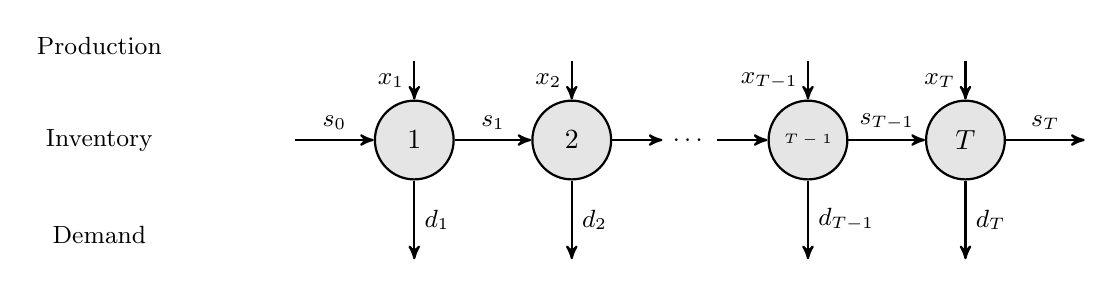
\begin{tikzpicture}[
    node distance=2cm, 
    thick, 
    >=stealth',
    every node/.style={font=\small},
    main/.style={circle, draw, fill=gray!20, minimum size=1cm, font=\normalsize}
]

% Nodes
\node[main] (1) {1};
\node[main, right of=1] (2) {2};
\node[right of=2, node distance=1.5cm] (dots) {\dots};
\node[main, right of=dots, node distance=1.5cm] (T1) {\tiny \(T-1\)};
\node[main, right of=T1] (T) {\(T\)};

% Arrows for Production
\foreach \i in {1,2,T}
    \draw[->] (\i) ++(0,1) -- node[left] {$x_\i$} (\i.north);
\foreach \i in {T1}
    \draw[->] (\i) ++(0,1) -- node[left] {$x_{T-1}$} (\i.north);
% Arrows for Inventory
\draw[<-] (1.west) -- ++(-1,0) node[midway, above] {$s_0$};
\draw[->] (1.east) -- node[midway, above] {$s_1$} (2.west);
\draw[->] (2.east) -- node[midway, above] {} (dots.west);
\draw[->] (dots.east) -- node[midway, above] {} (T1.west);
\draw[->] (T1.east) -- node[midway, above] {$s_{T-1}$} (T.west);
\draw[->] (T.east) -- ++(1,0) node[midway, above] {$s_T$};

% Arrows for Demand (using variables d_i)
\foreach \i in {1,2,T}
    \draw[->] (\i.south) -- ++(0,-1) node[midway, right] {$d_\i$};

\foreach \i in {T1}
    \draw[->] (\i.south) -- ++(0,-1) node[midway, right] {$d_{T-1}$};
% Labels
\node at (-4,1.2) {Production};
\node at (-4,0) {Inventory};
\node at (-4,-1.2) {Demand};

\end{tikzpicture}
\end{document}
